\section{Where the Model and the Data Disagree}
\label{sec:tension}

\subsection{What the data say}

The stock-level test of Section~\ref{sec:stock} found that stocks whose owners have \emph{similar} horizons are slightly \emph{more} volatile the next quarter. That is the pattern the Fractal Market Hypothesis predicts: concentrated horizons are fragile.

\subsection{What the model says}

An earlier version of our paper claimed that the model produced the same pattern, that narrowing the distribution of horizons both lowers horizon diversity and \emph{raises} volatility. We have now tested this properly and found that the claim was unsupported.

The earlier check built a narrower horizon distribution but then called the simulation routine, which drew its own horizons internally, so the narrower horizons never reached the simulated market. Whatever relationship appeared came from random variation between runs. We fixed this by feeding the narrower horizons into the actual simulation. We narrow each investor type's log-normal spread by dividing its $\sigma$ by a compression factor running from 0.5 (wider than baseline) to 3 (much narrower), and run 25 simulations at each factor for two clustering strengths.

\begin{table}[htbp]
\centering
\caption{Simulated volatility when the horizon distribution is compressed. Horizon diversity is computed with the fixed 16-bin definition (Eq.~\eqref{eq:tdi}). Volatility is multiplied by 1{,}000 for readability. 25 runs per cell.}
\label{tab:conc}
\begin{tabular}{lrrrrr}
\toprule
Compression factor & 0.5 & 1.0 & 1.5 & 2.0 & 3.0\\
\midrule
Horizon diversity & 2.52 & 2.44 & 2.29 & 2.17 & 2.01\\
Volatility, clustering strength 0.5 & 0.95 & 0.94 & 0.95 & 0.92 & 0.84\\
Volatility, clustering strength 2.0 & 0.86 & 0.88 & 0.79 & 0.80 & 0.80\\
\bottomrule
\end{tabular}
\end{table}

At clustering strength 0.5, volatility at the strongest compression is lower than at the weakest (Welch $t=-2.72$, $p=0.009$). At strength 2.0 the difference points the same way but is not significant ($p=0.13$). Across individual runs, horizon diversity and volatility are \emph{positively} correlated ($r=+0.21$, $p=0.02$ at strength 0.5; $r=+0.17$, $p=0.06$ at strength 2.0). Figure~\ref{fig:conc} shows this.

\begin{figure}[htbp]
\centering
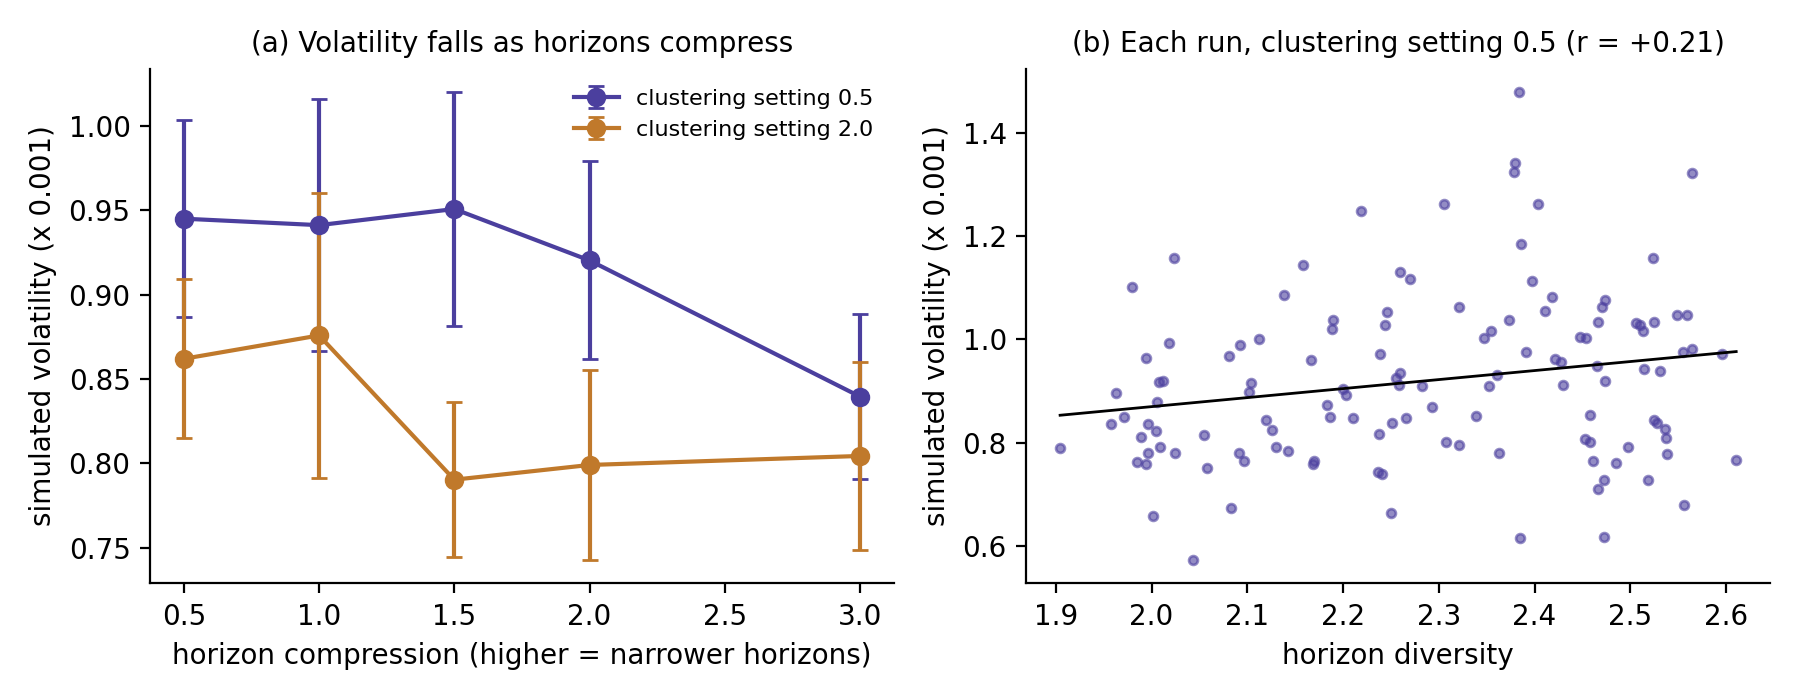
\includegraphics[width=0.95\linewidth]{conc_check}
\caption{(a) Simulated volatility against horizon compression for two clustering strengths (error bars are 95\% ranges for the mean). (b) Each simulation run at clustering strength 0.5: more diverse horizons go with slightly higher volatility.}
\label{fig:conc}
\end{figure}

\subsection{Why the model behaves this way}

The explanation is the friction channel of Eq.~\eqref{eq:sigeff}. When investors' horizons are close together, the average distance between an investor and their counterparties is small, so noise is low and volatility is lower. More diverse horizons mean more cross-horizon friction and more noise. The model contains \emph{no} mechanism by which concentrated horizons make the market \emph{fragile}: nothing weakens when diversity is lost, so nothing amplifies a shock. The fragility channel that the Fractal Market Hypothesis describes remains a verbal idea in our model, not something the simulation generates.

\begin{keyidea}[The tension in one sentence]
In the model, less diverse horizons \emph{reduce} volatility through lower friction; in the stock data, owners with similar horizons go with \emph{higher} volatility, a small effect in the direction the Fractal Market Hypothesis predicts but the opposite direction to the model's own simulated channel.
\end{keyidea}

We have corrected the paper to say this. We also note that the data effect is small and comes from a survivors-only sample, so it may not be reliable. The disagreement is real, but it does not by itself tell us which side is wrong.

\subsection{Options for the model}

If the aim is a model whose simulated behaviour agrees with the data, the model needs a channel through which the loss of horizon diversity makes the market fragile. We see three options.

\begin{description}[leftmargin=1.2em,style=nextline]
\item[Option A: a horizon-dependent stabiliser.] Make the value-investing force (the term with weight $\bar\alpha$ in Eq.~\eqref{eq:demand}) weaker when horizons are concentrated, representing the fact that long-horizon value investors are the ones who step in during a sell-off. \emph{For:} it directly produces the fragility the hypothesis describes, so model and data could agree. \emph{Against:} it requires re-verifying every simulation result, and because it is introduced after seeing the data it risks looking like building the answer we wanted. It must be reported openly as a post-hoc change.
\item[Option B: horizon-dependent liquidity.] Add a liquidity-provider role whose willingness to absorb trades depends on how many counterparties with different horizons are available, so that concentrated horizons reduce market depth and raise the price impact $\lambda$. \emph{For:} closer to the disagreement-and-volume mechanism of \citet{harrisraviv1993} and to the real way horizons are supposed to matter. \emph{Against:} a larger redesign with new parameters.
\item[Option C: keep the model and report the tension.] Describe the model as capturing only the friction channel, say plainly that the data point to a channel it does not contain, and treat that as an open question. \emph{For:} simple and honest. \emph{Against:} a weaker contribution, since the model then does not explain the stock-level evidence.
\end{description}

We have not chosen among these. We think the choice depends partly on how a referee would view post-hoc model changes, which is a question for experienced researchers in the field, and we are seeking advice on it.
